\documentclass[tikz,margin=1mm]{standalone}
\usetikzlibrary{matrix}
\tikzset{
    every matrix/.style={
        inner sep=-\pgflinewidth,
        matrix of math nodes,
        column sep=-\pgflinewidth,
        nodes={
            draw=black,
            font=\color{black},
            minimum size=.8cm,
            minimum width=1cm,
            anchor=center
        }
    }
}
\begin{document}
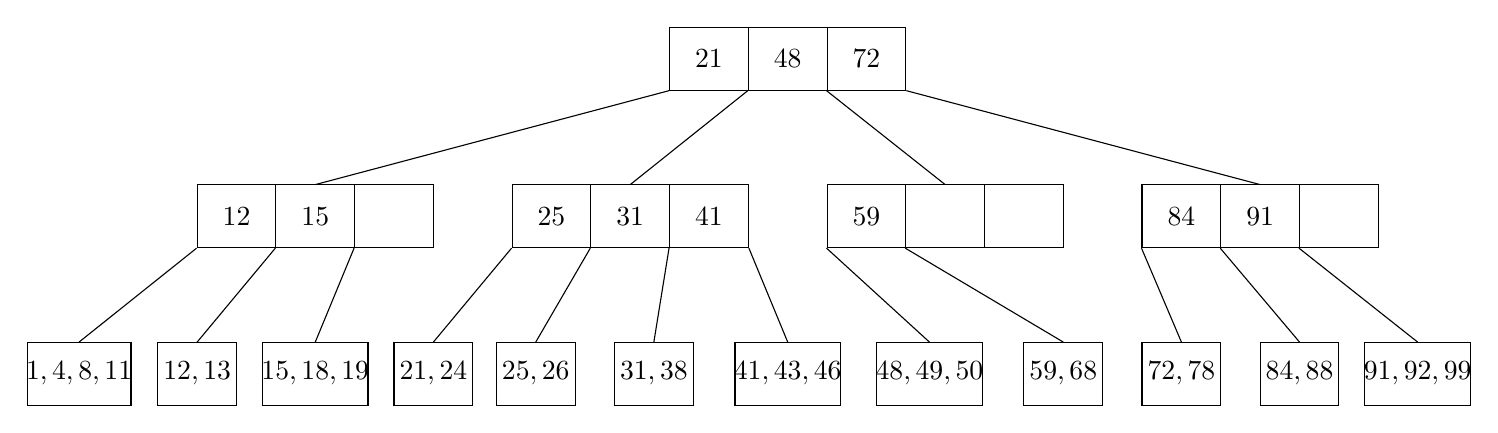
\begin{tikzpicture}
\matrix[above] (t1) at (0,0) {21 & 48 & 72\\};

\matrix[above] (t21) at (-6,-2) {12 & 15 & \quad\\};

\matrix[above] (t22) at (-2,-2) {25 & 31 & 41\\};

\matrix[above] (t23) at (2,-2) {59 & \quad & \quad\\};

\matrix[above] (t24) at (6,-2) {84 & 91 & \quad\\};

\matrix[above] (t31) at (-9,-4) {1, 4, 8, 11\\};

\matrix[above] (t32) at (-7.5,-4) {12, 13\\};

\matrix[above] (t33) at (-6,-4) {15, 18, 19\\};

\matrix[above] (t34) at (-4.5,-4) {21, 24\\};

\matrix[above] (t35) at (-3.2,-4) {25, 26\\};

\matrix[above] (t36) at (-1.7,-4) {31, 38\\};

\matrix[above] (t37) at (0,-4) {41, 43, 46\\};

\matrix[above] (t38) at (1.8,-4) {48, 49, 50\\};

\matrix[above] (t39) at (3.5,-4) {59, 68\\};

\matrix[above] (t310) at (5,-4) {72, 78\\};

\matrix[above] (t311) at (6.5,-4) {84, 88\\};

\matrix[above] (t312) at (8,-4) {91, 92, 99\\};

\draw[black]
    (t1-1-1.south west) -- (t21.north)
    (t1-1-2.south west) -- (t22.north)
    (t1-1-3.south west) -- (t23.north)
    (t1-1-3.south east) -- (t24.north)
    (t21-1-1.south west) -- (t31.north)
    (t21-1-2.south west) -- (t32.north)
    (t21-1-3.south west) -- (t33.north)
    (t22-1-1.south west) -- (t34.north)
    (t22-1-2.south west) -- (t35.north)
    (t22-1-3.south west) -- (t36.north)
    (t22-1-3.south east) -- (t37.north)
    (t23-1-1.south west) -- (t38.north)
    (t23-1-2.south west) -- (t39.north)
    (t24-1-1.south west) -- (t310.north)
    (t24-1-2.south west) -- (t311.north)
    (t24-1-3.south west) -- (t312.north);
\end{tikzpicture}
\end{document}